% Name: Training and validation loss
% Description: Training and validation loss over the epochs of a training run, with the epoch of lowest validation loss marked, as results sections often show.
% Tags: line plot, machine learning, loss curve, overfitting

\usepackage{pgfplots}
\pgfplotsset{compat=1.18}

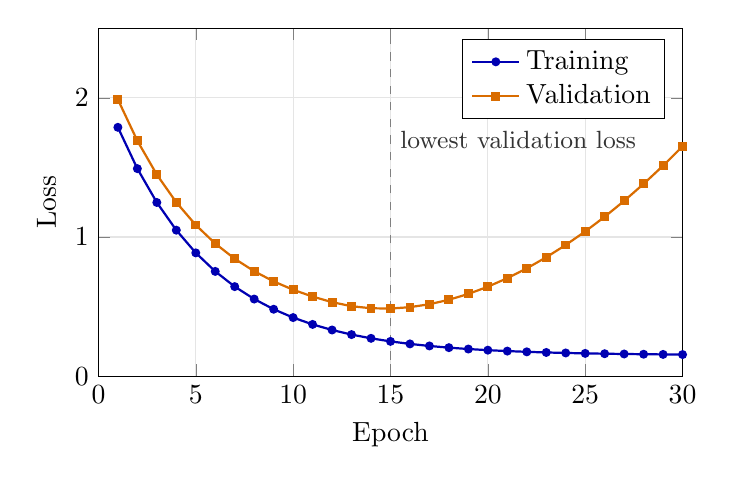
\begin{tikzpicture}
  \begin{axis}[
    width=9cm, height=6cm, xlabel=Epoch, ylabel=Loss,
    xmin=0, xmax=30, ymin=0, ymax=2.5,
    legend pos=north east, legend cell align=left,
    grid=major, grid style={gray!20}, domain=1:30, samples=30,
  ]
    \addplot[thick, blue!70!black, mark=*, mark size=1.2pt] {0.15 + 2*exp(-x/5)};
    \addplot[thick, orange!85!black, mark=square*, mark size=1.2pt] {0.35 + 2*exp(-x/5) + 0.004*(x-12)^2*(x>12)};
    % The validation loss is lowest near epoch 15, where it starts to rise again.
    \draw[dashed, gray] (axis cs:15,0) -- (axis cs:15,2.5);
    \node[right, font=\small, gray!40!black] at (axis cs:15,1.7) {lowest validation loss};
    \legend{Training, Validation}
  \end{axis}
\end{tikzpicture}
